% Options for packages loaded elsewhere
\PassOptionsToPackage{unicode}{hyperref}
\PassOptionsToPackage{hyphens}{url}
\PassOptionsToPackage{dvipsnames,svgnames,x11names}{xcolor}
%
\documentclass[
  letterpaper,
  DIV=11,
  numbers=noendperiod]{scrreprt}

\usepackage{amsmath,amssymb}
\usepackage{lmodern}
\usepackage{iftex}
\ifPDFTeX
  \usepackage[T1]{fontenc}
  \usepackage[utf8]{inputenc}
  \usepackage{textcomp} % provide euro and other symbols
\else % if luatex or xetex
  \usepackage{unicode-math}
  \defaultfontfeatures{Scale=MatchLowercase}
  \defaultfontfeatures[\rmfamily]{Ligatures=TeX,Scale=1}
\fi
% Use upquote if available, for straight quotes in verbatim environments
\IfFileExists{upquote.sty}{\usepackage{upquote}}{}
\IfFileExists{microtype.sty}{% use microtype if available
  \usepackage[]{microtype}
  \UseMicrotypeSet[protrusion]{basicmath} % disable protrusion for tt fonts
}{}
\makeatletter
\@ifundefined{KOMAClassName}{% if non-KOMA class
  \IfFileExists{parskip.sty}{%
    \usepackage{parskip}
  }{% else
    \setlength{\parindent}{0pt}
    \setlength{\parskip}{6pt plus 2pt minus 1pt}}
}{% if KOMA class
  \KOMAoptions{parskip=half}}
\makeatother
\usepackage{xcolor}
\setlength{\emergencystretch}{3em} % prevent overfull lines
\setcounter{secnumdepth}{5}
% Make \paragraph and \subparagraph free-standing
\ifx\paragraph\undefined\else
  \let\oldparagraph\paragraph
  \renewcommand{\paragraph}[1]{\oldparagraph{#1}\mbox{}}
\fi
\ifx\subparagraph\undefined\else
  \let\oldsubparagraph\subparagraph
  \renewcommand{\subparagraph}[1]{\oldsubparagraph{#1}\mbox{}}
\fi

\usepackage{color}
\usepackage{fancyvrb}
\newcommand{\VerbBar}{|}
\newcommand{\VERB}{\Verb[commandchars=\\\{\}]}
\DefineVerbatimEnvironment{Highlighting}{Verbatim}{commandchars=\\\{\}}
% Add ',fontsize=\small' for more characters per line
\usepackage{framed}
\definecolor{shadecolor}{RGB}{241,243,245}
\newenvironment{Shaded}{\begin{snugshade}}{\end{snugshade}}
\newcommand{\AlertTok}[1]{\textcolor[rgb]{0.68,0.00,0.00}{#1}}
\newcommand{\AnnotationTok}[1]{\textcolor[rgb]{0.37,0.37,0.37}{#1}}
\newcommand{\AttributeTok}[1]{\textcolor[rgb]{0.40,0.45,0.13}{#1}}
\newcommand{\BaseNTok}[1]{\textcolor[rgb]{0.68,0.00,0.00}{#1}}
\newcommand{\BuiltInTok}[1]{\textcolor[rgb]{0.00,0.23,0.31}{#1}}
\newcommand{\CharTok}[1]{\textcolor[rgb]{0.13,0.47,0.30}{#1}}
\newcommand{\CommentTok}[1]{\textcolor[rgb]{0.37,0.37,0.37}{#1}}
\newcommand{\CommentVarTok}[1]{\textcolor[rgb]{0.37,0.37,0.37}{\textit{#1}}}
\newcommand{\ConstantTok}[1]{\textcolor[rgb]{0.56,0.35,0.01}{#1}}
\newcommand{\ControlFlowTok}[1]{\textcolor[rgb]{0.00,0.23,0.31}{#1}}
\newcommand{\DataTypeTok}[1]{\textcolor[rgb]{0.68,0.00,0.00}{#1}}
\newcommand{\DecValTok}[1]{\textcolor[rgb]{0.68,0.00,0.00}{#1}}
\newcommand{\DocumentationTok}[1]{\textcolor[rgb]{0.37,0.37,0.37}{\textit{#1}}}
\newcommand{\ErrorTok}[1]{\textcolor[rgb]{0.68,0.00,0.00}{#1}}
\newcommand{\ExtensionTok}[1]{\textcolor[rgb]{0.00,0.23,0.31}{#1}}
\newcommand{\FloatTok}[1]{\textcolor[rgb]{0.68,0.00,0.00}{#1}}
\newcommand{\FunctionTok}[1]{\textcolor[rgb]{0.28,0.35,0.67}{#1}}
\newcommand{\ImportTok}[1]{\textcolor[rgb]{0.00,0.46,0.62}{#1}}
\newcommand{\InformationTok}[1]{\textcolor[rgb]{0.37,0.37,0.37}{#1}}
\newcommand{\KeywordTok}[1]{\textcolor[rgb]{0.00,0.23,0.31}{#1}}
\newcommand{\NormalTok}[1]{\textcolor[rgb]{0.00,0.23,0.31}{#1}}
\newcommand{\OperatorTok}[1]{\textcolor[rgb]{0.37,0.37,0.37}{#1}}
\newcommand{\OtherTok}[1]{\textcolor[rgb]{0.00,0.23,0.31}{#1}}
\newcommand{\PreprocessorTok}[1]{\textcolor[rgb]{0.68,0.00,0.00}{#1}}
\newcommand{\RegionMarkerTok}[1]{\textcolor[rgb]{0.00,0.23,0.31}{#1}}
\newcommand{\SpecialCharTok}[1]{\textcolor[rgb]{0.37,0.37,0.37}{#1}}
\newcommand{\SpecialStringTok}[1]{\textcolor[rgb]{0.13,0.47,0.30}{#1}}
\newcommand{\StringTok}[1]{\textcolor[rgb]{0.13,0.47,0.30}{#1}}
\newcommand{\VariableTok}[1]{\textcolor[rgb]{0.07,0.07,0.07}{#1}}
\newcommand{\VerbatimStringTok}[1]{\textcolor[rgb]{0.13,0.47,0.30}{#1}}
\newcommand{\WarningTok}[1]{\textcolor[rgb]{0.37,0.37,0.37}{\textit{#1}}}

\providecommand{\tightlist}{%
  \setlength{\itemsep}{0pt}\setlength{\parskip}{0pt}}\usepackage{longtable,booktabs,array}
\usepackage{calc} % for calculating minipage widths
% Correct order of tables after \paragraph or \subparagraph
\usepackage{etoolbox}
\makeatletter
\patchcmd\longtable{\par}{\if@noskipsec\mbox{}\fi\par}{}{}
\makeatother
% Allow footnotes in longtable head/foot
\IfFileExists{footnotehyper.sty}{\usepackage{footnotehyper}}{\usepackage{footnote}}
\makesavenoteenv{longtable}
\usepackage{graphicx}
\makeatletter
\def\maxwidth{\ifdim\Gin@nat@width>\linewidth\linewidth\else\Gin@nat@width\fi}
\def\maxheight{\ifdim\Gin@nat@height>\textheight\textheight\else\Gin@nat@height\fi}
\makeatother
% Scale images if necessary, so that they will not overflow the page
% margins by default, and it is still possible to overwrite the defaults
% using explicit options in \includegraphics[width, height, ...]{}
\setkeys{Gin}{width=\maxwidth,height=\maxheight,keepaspectratio}
% Set default figure placement to htbp
\makeatletter
\def\fps@figure{htbp}
\makeatother
\newlength{\cslhangindent}
\setlength{\cslhangindent}{1.5em}
\newlength{\csllabelwidth}
\setlength{\csllabelwidth}{3em}
\newlength{\cslentryspacingunit} % times entry-spacing
\setlength{\cslentryspacingunit}{\parskip}
\newenvironment{CSLReferences}[2] % #1 hanging-ident, #2 entry spacing
 {% don't indent paragraphs
  \setlength{\parindent}{0pt}
  % turn on hanging indent if param 1 is 1
  \ifodd #1
  \let\oldpar\par
  \def\par{\hangindent=\cslhangindent\oldpar}
  \fi
  % set entry spacing
  \setlength{\parskip}{#2\cslentryspacingunit}
 }%
 {}
\usepackage{calc}
\newcommand{\CSLBlock}[1]{#1\hfill\break}
\newcommand{\CSLLeftMargin}[1]{\parbox[t]{\csllabelwidth}{#1}}
\newcommand{\CSLRightInline}[1]{\parbox[t]{\linewidth - \csllabelwidth}{#1}\break}
\newcommand{\CSLIndent}[1]{\hspace{\cslhangindent}#1}

\usepackage{booktabs}
\usepackage{longtable}
\usepackage{array}
\usepackage{multirow}
\usepackage{wrapfig}
\usepackage{float}
\usepackage{colortbl}
\usepackage{pdflscape}
\usepackage{tabu}
\usepackage{threeparttable}
\usepackage{threeparttablex}
\usepackage[normalem]{ulem}
\usepackage{makecell}
\usepackage{xcolor}
- \usepackage{lscape}
- \newcommand{\blandscape}{\begin{landscape}}
- \newcommand{\elandscape}{\end{landscape}}
- \usepackage{xunicode}
- \usepackage{geometry}
- \usepackage{paralist}
- \geometry{a4paper,right=1.2in, left=1.2in}
- \geometry{twoside}
- \renewcommand{\baselinestretch}{1.2} 
- \setmainfont[Scale=1.1]{ChulaCharasNew}
- \setmonofont[Scale=0.7]{Courier New}
- \setlength{\parindent}{2em}
- \XeTeXlinebreaklocale "th"
- \XeTeXlinebreakskip = 0pt plus 1.2pt
- \XeTeXlinebreaklocale "th_TH"
- \usepackage{booktabs}
- \usepackage{longtable}
- \usepackage{array}
- \usepackage{multirow}
- \usepackage{wrapfig}
- \usepackage{colortbl}
- \usepackage{pdflscape}
- \usepackage{tabu}
- \usepackage{threeparttable}
- \usepackage{threeparttablex}
- \usepackage[normalem]{ulem}
- \usepackage{makecell}
- \usepackage{xcolor}
\KOMAoption{captions}{tableheading}
\makeatletter
\makeatother
\makeatletter
\@ifpackageloaded{bookmark}{}{\usepackage{bookmark}}
\makeatother
\makeatletter
\@ifpackageloaded{caption}{}{\usepackage{caption}}
\AtBeginDocument{%
\ifdefined\contentsname
  \renewcommand*\contentsname{Table of contents}
\else
  \newcommand\contentsname{Table of contents}
\fi
\ifdefined\listfigurename
  \renewcommand*\listfigurename{List of Figures}
\else
  \newcommand\listfigurename{List of Figures}
\fi
\ifdefined\listtablename
  \renewcommand*\listtablename{List of Tables}
\else
  \newcommand\listtablename{List of Tables}
\fi
\ifdefined\figurename
  \renewcommand*\figurename{Figure}
\else
  \newcommand\figurename{Figure}
\fi
\ifdefined\tablename
  \renewcommand*\tablename{Table}
\else
  \newcommand\tablename{Table}
\fi
}
\@ifpackageloaded{float}{}{\usepackage{float}}
\floatstyle{ruled}
\@ifundefined{c@chapter}{\newfloat{codelisting}{h}{lop}}{\newfloat{codelisting}{h}{lop}[chapter]}
\floatname{codelisting}{Listing}
\newcommand*\listoflistings{\listof{codelisting}{List of Listings}}
\makeatother
\makeatletter
\@ifpackageloaded{caption}{}{\usepackage{caption}}
\@ifpackageloaded{subcaption}{}{\usepackage{subcaption}}
\makeatother
\makeatletter
\@ifpackageloaded{tcolorbox}{}{\usepackage[many]{tcolorbox}}
\makeatother
\makeatletter
\@ifundefined{shadecolor}{\definecolor{shadecolor}{rgb}{.97, .97, .97}}
\makeatother
\makeatletter
\makeatother
\ifLuaTeX
  \usepackage{selnolig}  % disable illegal ligatures
\fi
\IfFileExists{bookmark.sty}{\usepackage{bookmark}}{\usepackage{hyperref}}
\IfFileExists{xurl.sty}{\usepackage{xurl}}{} % add URL line breaks if available
\urlstyle{same} % disable monospaced font for URLs
\hypersetup{
  pdftitle={หน่วยที่ 4 การเตรียมข้อมูล},
  pdfauthor={ผศ.ดร.สิวะโชติ ศรีสุทธิยากร},
  colorlinks=true,
  linkcolor={blue},
  filecolor={Maroon},
  citecolor={Blue},
  urlcolor={Blue},
  pdfcreator={LaTeX via pandoc}}

\title{หน่วยที่ 4 การเตรียมข้อมูล}
\author{ผศ.ดร.สิวะโชติ ศรีสุทธิยากร}
\date{10/29/2022}

\begin{document}
\maketitle
\ifdefined\Shaded\renewenvironment{Shaded}{\begin{tcolorbox}[enhanced, borderline west={3pt}{0pt}{shadecolor}, interior hidden, frame hidden, breakable, sharp corners, boxrule=0pt]}{\end{tcolorbox}}\fi

\renewcommand*\contentsname{Table of contents}
{
\hypersetup{linkcolor=}
\setcounter{tocdepth}{2}
\tableofcontents
}
\bookmarksetup{startatroot}

\hypertarget{uxe41uxe1cuxe19uxe01uxe32uxe23uxe2auxe2duxe19uxe1buxe23uxe30uxe08uxe33uxe2buxe19uxe27uxe22}{%
\chapter*{แผนการสอนประจำหน่วย}\label{uxe41uxe1cuxe19uxe01uxe32uxe23uxe2auxe2duxe19uxe1buxe23uxe30uxe08uxe33uxe2buxe19uxe27uxe22}}
\addcontentsline{toc}{chapter}{แผนการสอนประจำหน่วย}

\hypertarget{uxe0auxe14uxe27uxe0auxe32}{%
\subsection*{\texorpdfstring{\textbf{ชุดวิชา}}{ชุดวิชา}}\label{uxe0auxe14uxe27uxe0auxe32}}
\addcontentsline{toc}{subsection}{\textbf{ชุดวิชา}}

หลักวิทยาการข้อมูลและการแสดงผลด้วยแผนภาพ

\hypertarget{uxe2buxe19uxe27uxe22uxe17-4}{%
\subsection*{\texorpdfstring{\textbf{หน่วยที่
4}}{หน่วยที่ 4}}\label{uxe2buxe19uxe27uxe22uxe17-4}}
\addcontentsline{toc}{subsection}{\textbf{หน่วยที่ 4}}

การเตรียมข้อมูล

\hypertarget{uxe15uxe2duxe19uxe17}{%
\subsection*{\texorpdfstring{\textbf{ตอนที่}}{ตอนที่}}\label{uxe15uxe2duxe19uxe17}}
\addcontentsline{toc}{subsection}{\textbf{ตอนที่}}

4.1 การจัดระเบียบข้อมูล

4.2 การจัดกระทำข้อมูล

4.3 การวิเคราะห์เพื่อสำรวจข้อมูลและการแก้ปัญหา

\hypertarget{uxe41uxe19uxe27uxe04uxe14}{%
\subsection*{\texorpdfstring{\textbf{แนวคิด}}{แนวคิด}}\label{uxe41uxe19uxe27uxe04uxe14}}
\addcontentsline{toc}{subsection}{\textbf{แนวคิด}}

ขั้นตอนการดำเนินงานทางด้านวิทยาการข้อมูลอาจจำแนกออกเป็น 5 ขั้นตอนใหญ่ได้แก่
การระบุปัญหา/วัตถุประสงค์ของงาน การเก็บรวบรวมข้อมูล การเตรียมข้อมูล
การวิเคราะห์ข้อมูล/การพัฒนาโมเดล และการนำผลการวิเคราะห์/โมเดลไปใช้งาน

ส่วนประกอบสำคัญที่สุดในการดำเนินงานทางด้านสถิติและวิทยาการข้อมูลคือข้อมูล
ถึงแม้ว่าปัจจุบันข้อมูลจะเป็นทรัพยากรที่มีอยู่จำนวนมาก และสามารถเข้าถึงได้โดยง่าย
แต่ในสถานการณ์ของการทำงานจริง
ข้อมูลส่วนใหญ่มักยังไม่อยู่ในสภาพที่พร้อมสำหรับการนำไปดำเนินการวิเคราะห์ตามวัตถุประสงค์ต่าง
ๆ การเตรียมข้อมูลจึงเป็นขั้นตอนสำคัญที่นักสถิติและนักวิทยาการข้อมูลต้องดำเนินการ
เพื่อจัดระเบียบหรือจัดกระทำข้อมูล
ในเชิงปฏิบัติการเตรียมข้อมูลเป็นขั้นตอนที่ใช้ทรัพยากรและเวลาค่อนข้างมาก
กล่าวกันว่าขั้นตอนนี้ใช้เวลาในการดำเนินงานคิดเป็นกว่าร้อยละ 80
ของการดำเนินงานทั้งหมดของโครงการวิทยาการข้อมูล (Dasu, \& Johnson, 2003)
นอกจากนี้การเตรียมข้อมูลนี้ยังมีลักษณะการดำเนินงานเป็นแบบทวนซ้ำไปมาหลายครั้ง
และไม่ได้มีรูปแบบการดำเนินงานที่ตายตัวเหมือนกันในแต่ละโครงการ
ความรู้และทักษะนี้จึงมีความจำเป็นอย่างยิ่งสำหรับนักสถิติและนักวิทยาการข้อมูล

เพื่อให้ผู้อ่านมีความรู้และทักษะที่เพียงพอสำหรับการเตรียมข้อมูล
เนื้อหาภายในหน่วยการเรียนนี้จึงประกอบด้วย
มโนทัศน์และวิธีการที่จำเป็นสำหรับการเตรียมข้อมูลดังกล่าว ประกอบด้วย การจัดระเบียบชุดข้อมูล
การจัดกระทำข้อมูล การวิเคราะห์เพื่อสำรวจข้อมูล และการแก้ปัญหาที่เกิดขึ้นในข้อมูลได้แก่
ปัญหาค่าสูญหาย และปัญหาค่าผิดปกติ

\hypertarget{uxe27uxe15uxe16uxe1buxe23uxe30uxe2auxe07uxe04}{%
\subsection*{\texorpdfstring{\textbf{วัตถุประสงค์}}{วัตถุประสงค์}}\label{uxe27uxe15uxe16uxe1buxe23uxe30uxe2auxe07uxe04}}
\addcontentsline{toc}{subsection}{\textbf{วัตถุประสงค์}}

เมื่อศึกษาหน่วยที่ 4 จบแล้วผู้อ่านสามารถ

\begin{enumerate}
\def\labelenumi{\arabic{enumi}.}
\tightlist
\item
  อธิบายมโนทัศน์ของชุดข้อมูลจัดระเบียบ
\item
  สามารถสำรวจสภาพและระบุปัญหาที่เกิดขึ้นในชุดข้อมูล โดยใช้สถิติพื้นฐานและทัศนภาพข้อมูล
\item
  สามารถจัดระเบียบชุดข้อมูลให้อยู่ในรูปแบบตารางข้อมูลที่เหมาะสมสำหรับการวิเคราะห์ข้อมูล
\item
  สามารถจัดกระทำข้อมูลเพื่อให้ได้ชุดข้อมูลที่เหมาะสมและตรงกับความต้องการในการวิเคราะห์ข้อมูล
\item
  อธิบายมโนทัศน์ของค่าสูญหายได้ สามารถวิเคราะห์และทดแทนค่าสูญหายได้อย่างเหมาะสม
\item
  อธิบายมโนทัศน์ของค่าผิดปกติได้ สามารถวิเคราะห์และแก้ปัญหาค่าผิดปกติได้อย่างเหมาะสม
\end{enumerate}

\bookmarksetup{startatroot}

\hypertarget{uxe15uxe2duxe19uxe17-4.1-uxe01uxe32uxe23uxe08uxe14uxe23uxe30uxe40uxe1auxe22uxe1auxe02uxe2duxe21uxe25-tidying-data}{%
\chapter*{ตอนที่ 4.1 การจัดระเบียบข้อมูล (tidying
data)}\label{uxe15uxe2duxe19uxe17-4.1-uxe01uxe32uxe23uxe08uxe14uxe23uxe30uxe40uxe1auxe22uxe1auxe02uxe2duxe21uxe25-tidying-data}}
\addcontentsline{toc}{chapter}{ตอนที่ 4.1 การจัดระเบียบข้อมูล (tidying data)}

ชุดข้อมูล (data set) มีลักษณะเป็นตารางที่ประกอบด้วยมิติด้านคอลัมน์ (column) และแถว
(row) ใช้เก็บข้อมูลของตัวแปรต่าง ๆ
ข้อมูลที่ถูกจัดเก็บอยู่ในตารางดังกล่าวเป็นไปได้ทั้งข้อมูลเชิงปริมาณที่มีค่าเป็นตัวเลข
ข้อมูลเชิงคุณลักษณะที่ไม่ใช่ตัวเลข
การออกแบบตารางสำหรับจัดเก็บข้อมูลนั้นสามารถทำได้หลากหลายลักษณะ
พิจารณาชุดข้อมูลในตาราง 1 และ 2
ด้านล่างจะเห็นว่าถึงแม้จะเป็นเป็นชุดข้อมูลที่จัดเก็บข้อมูลเดียวกัน
แต่ก็สามารถที่จะมีรูปแบบการจัดเก็บที่แตกต่างกันได้

\textbf{ตาราง 1} : คะแนนสอบวิชาคณิตศาสตร์และภาษาอังกฤษของนักเรียน (รูปแบบที่ 1)

\begingroup\fontsize{15}{17}\selectfont

\begin{tabular}{l|r|r}
\hline
นักเรียน & คะแนนวิชาคณิตศาสตร์ & คะแนนวิชาวิทยาศาสตร์\\
\hline
บุญมา & 10 & 2\\
\hline
บุญมี & NA & 20\\
\hline
บุญเติม & 15 & 20\\
\hline
บุญหนัก & 4 & 5\\
\hline
\end{tabular}
\endgroup{}

\textbf{ตาราง 2} : คะแนนสอบวิชาคณิตศาสตร์และภาษาอังกฤษของนักเรียน (รูปแบบที่ 2)

\begingroup\fontsize{15}{17}\selectfont

\begin{tabular}{l|l|r}
\hline
นักเรียน & รายวิชา & คะแนน\\
\hline
บุญมา & คณิตศาสตร์ & 10\\
\hline
บุญมา & ภาษาอังกฤษ & 2\\
\hline
บุญมี & คณิตศาสตร์ & NA\\
\hline
บุญมี & ภาษาอังกฤษ & 20\\
\hline
บุญเติม & คณิตศาสตร์ & 15\\
\hline
บุญเติม & ภาษาอังกฤษ & 20\\
\hline
บุญหนัก & คณิตศาสตร์ & 4\\
\hline
บุญหนัก & ภาษาอังกฤษ & 5\\
\hline
\end{tabular}
\endgroup{}

อย่างไรก็ตามการจัดเก็บข้อมูลในชุดข้อมูลในรูปแบบที่เหมาะสมกับการดำเนินการวิเคราะห์ข้อมูล
หรือการสร้างทัศนภาพข้อมูลจะช่วยให้การวิเคราะห์ข้อมูลตามวัตถุประสงค์ต่าง ๆ
สามารถทำได้ง่ายและมีประสิทธิภาพ
ในทางกลับกันการจัดเก็บข้อมูลในรูปแบบที่ไม่เหมาะสมจะเป็นอุปสรรคในการวิเคราะห์ข้อมูล
นอกจากนี้ยังอาจเป็นปัจจัยที่ก่อให้เกิดความผิดพลาดในผลการวิเคราะห์อีกด้วย
รูปแบบของชุดข้อมูลที่เหมาะสมและสนับสนุนให้การวิเคราะห์ข้อมูลสามารถดำเนินไปได้อย่างมีประสิทธิภาพเรียกว่า
\textbf{ชุดข้อมูลจัดระเบียบ (tidy data)}

ชุดข้อมูลจัดระเบียบเป็นตารางข้อมูลที่มีลักษณะสำคัญของรูปแบบการจัดเก็บข้อมูล 3 ประการ
(สิวะโชติ ศรีสุทธิยากร, 2564; Wickham, 2014) ดังนี้

\begin{enumerate}
\def\labelenumi{\arabic{enumi}.}
\tightlist
\item
  มิติด้านคอลัมน์ (column) ของชุดข้อมูล เป็นมิติของตัวแปร
  โดยที่แต่ละคอลมน์จะใช้เก็บข้อมูลตัวแปรได้เพียงคอลัมน์ละหนึ่งตัวแปรเท่านั้น
\item
  มิติด้านแถว (row) ของชุดข้อมูล เป็นมิติของหน่วยข้อมูล
  โดยที่แต่ละแถวจะใช้เก็บข้อมูลของหน่วยข้อมูลได้เพียงแถวละหนึ่งหน่วยข้อมูลเท่านั้น
\item
  ภายในแต่ละเซลล์ (cell) ของชุดข้อมูล จะใช้เก็บข้อมูลค่าสังเกตได้เพียงค่าเดียวเท่านั้น
\end{enumerate}

รูป 4.1 แสดงตัวอย่างของชุดข้อมูลจัดระเบียบที่มีคุณลักษณะข้างต้น สังเกตว่าหัวตาราง
(แถวแรกของตาราง) จะเป็นส่วนที่ใช้ระบุชื่อของตัวแปรในแต่ละคอลัมน์
อย่างไรก็ตามในสถานการณ์จริงชุดข้อมูลส่วนใหญ่มักมีลักษณะที่ละเมิดเงื่อนไขของชุดข้อมูลจัดระเบียบข้างต้นอย่างน้อยหนึ่งข้อ
การจัดระเบียบชุดข้อมูลจึงเป็นขั้นตอนที่มีความสำคัญภายใต้การดำเนินงานทางด้านวิทยาการข้อมูล
เนื้อหาในตอนที่ 4.1 นี้จึงจะกล่าวถึง การสำรวจลักษณะของชุดข้อมูล
เพื่อวิเคราะห์สภาพและระบุปัญหาความไม่เป็นระเบียบของชุดข้อมูล (ถ้ามี)
จากนั้นจะกล่าวถึงวิธีการที่เกี่ยวข้องสำหรับแก้ปัญหาดังกล่าว รายละเอียดมีดังนี้

\begin{figure}

{\centering 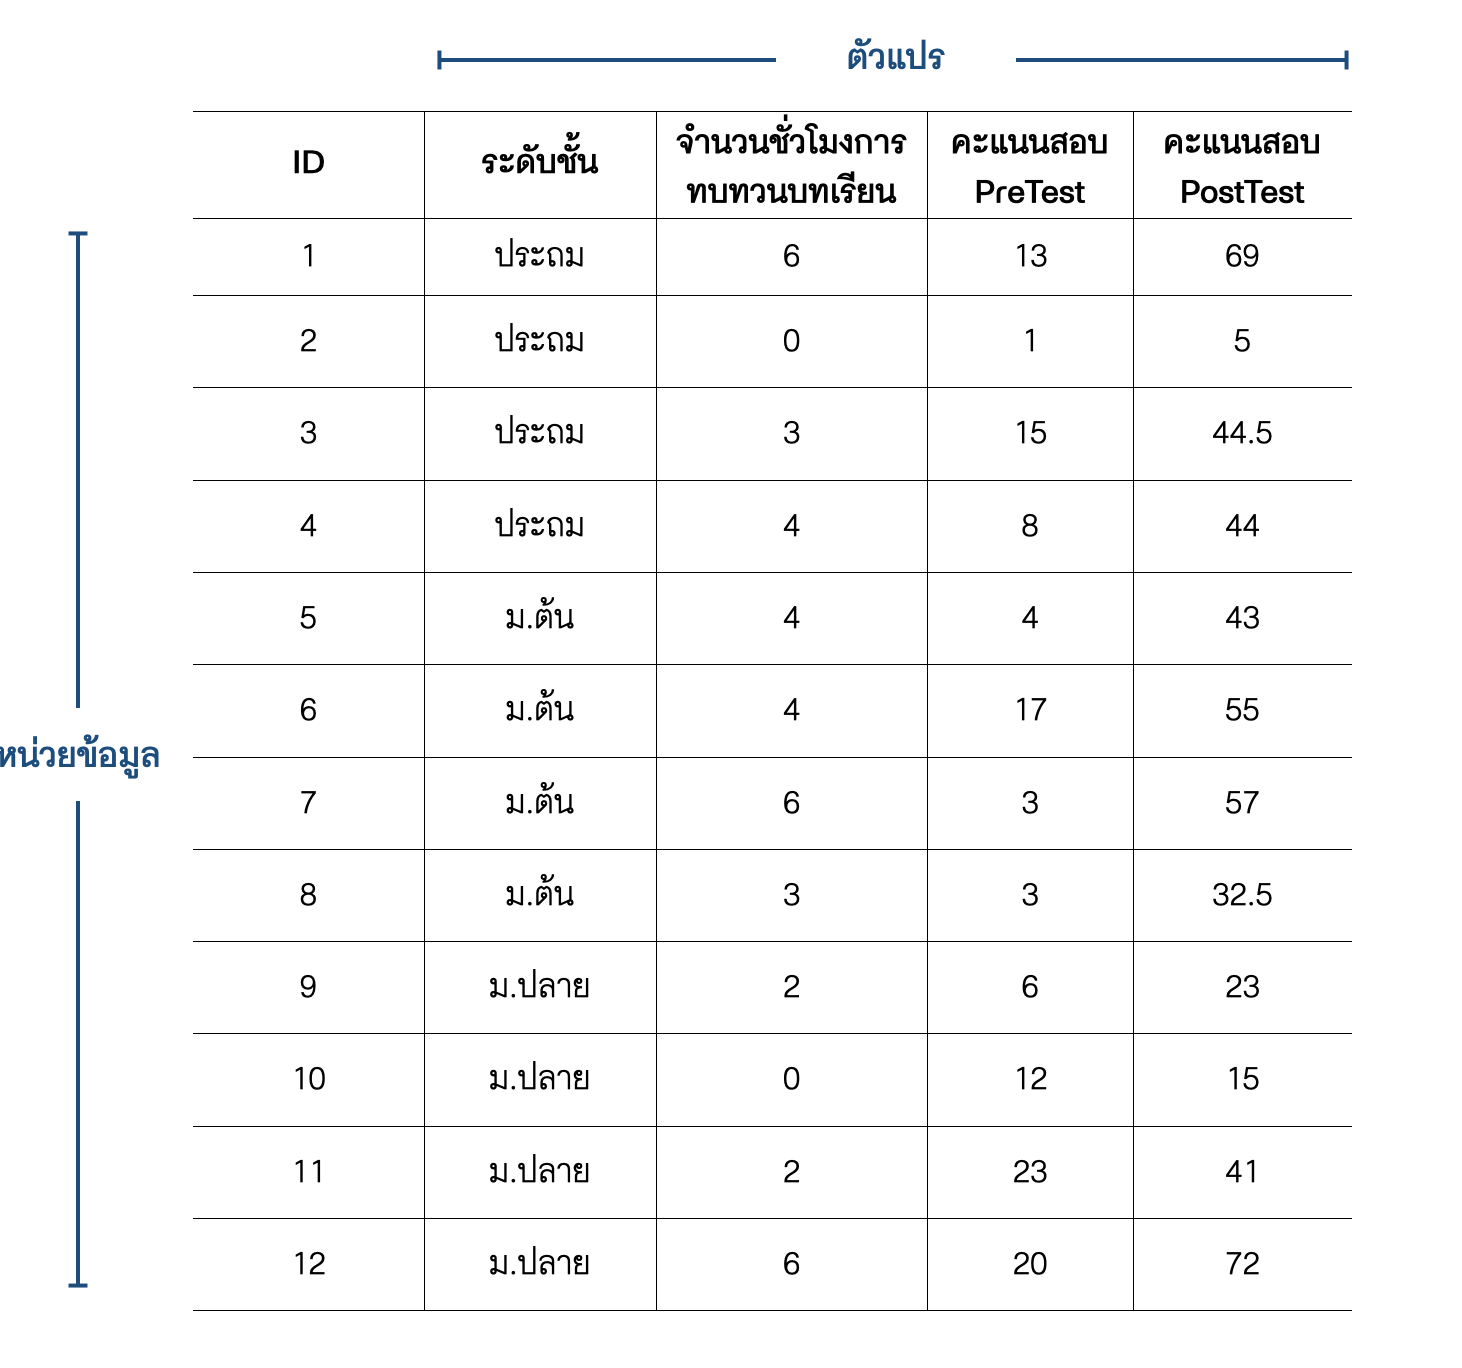
\includegraphics[width=1\textwidth,height=\textheight]{./tidydata.png}

}

\caption{รูป 4.1 ตัวอย่างข้อมูลจัดระเบียบ}

\end{figure}

\hypertarget{uxe40uxe23uxe2duxe07uxe17-4.1.1-uxe01uxe32uxe23uxe2auxe33uxe23uxe27uxe08uxe25uxe01uxe29uxe13uxe30uxe02uxe2duxe07uxe0auxe14uxe02uxe2duxe21uxe25}{%
\section*{เรื่องที่ 4.1.1
การสำรวจลักษณะของชุดข้อมูล}\label{uxe40uxe23uxe2duxe07uxe17-4.1.1-uxe01uxe32uxe23uxe2auxe33uxe23uxe27uxe08uxe25uxe01uxe29uxe13uxe30uxe02uxe2duxe07uxe0auxe14uxe02uxe2duxe21uxe25}}
\addcontentsline{toc}{section}{เรื่องที่ 4.1.1 การสำรวจลักษณะของชุดข้อมูล}

ในหัวข้อนี้จะใช้ชุดข้อมูล \texttt{gapminder} (Bryan, 2017)
ที่ประกอบด้วยข้อมูลเกี่ยวกับจำนวนประชากร (pop) ผลิตภัณฑ์มวลรวมในประเทศต่อหัว
(gdpPercap) และอายุขัยเฉลี่ยของประชากร (lifeExp) ของประเทศต่าง ๆ
เป็นตัวอย่างประกอบการอธิบาย เมื่อผู้วิเคราะห์นำข้อมูล \texttt{gapminder}
เข้าสู่โปรแกรมแล้วเรียกดูชุดข้อมูลจะได้ผลลัพธ์เป็นดังนี้

\begin{verbatim}
# A tibble: 1,704 x 6
   country     continent  year lifeExp      pop gdpPercap
   <fct>       <fct>     <int>   <dbl>    <int>     <dbl>
 1 Afghanistan Asia       1952    28.8  8425333      779.
 2 Afghanistan Asia       1957    30.3  9240934      821.
 3 Afghanistan Asia       1962    32.0 10267083      853.
 4 Afghanistan Asia       1967    34.0 11537966      836.
 5 Afghanistan Asia       1972    36.1 13079460      740.
 6 Afghanistan Asia       1977    38.4 14880372      786.
 7 Afghanistan Asia       1982    39.9 12881816      978.
 8 Afghanistan Asia       1987    40.8 13867957      852.
 9 Afghanistan Asia       1992    41.7 16317921      649.
10 Afghanistan Asia       1997    41.8 22227415      635.
# ... with 1,694 more rows
\end{verbatim}

\textbf{ตาราง 3} : จำนวนนักเรียนจำแนกตามรายวิชาและช่วงคะแนนผลการสอบ O-NET
ระดับชั้น ม.6 ปีการศึกษา 2560

\begingroup\fontsize{14}{16}\selectfont

\begin{tabu} to \linewidth {>{\raggedright}X>{\raggedleft}X>{\raggedleft}X>{\raggedleft}X>{\raggedleft}X>{\raggedleft}X>{\raggedleft}X>{\raggedleft}X>{\raggedleft}X>{\raggedleft}X>{\raggedleft}X}
\hline
\multicolumn{1}{c|}{ } & \multicolumn{10}{c}{ช่วงคะแนนผลสอบ O-NET} \\
\cline{2-11}
วิชา & < 10 คะแนน & 10-20 & 20-30 & 30-40 & 40-50 & 50-60 & 60-70 & 70-80 & 80-90 & 90-100\\
\hline
ภาษาไทย & 205 & 10918 & 39277 & 59459 & 80767 & 84977 & 61052 & 28544 & 6623 & 221\\
\hline
สังคมศึกษา & 93 & 11450 & 119492 & 155338 & 64380 & 17638 & 3721 & 447 & 8 & 0\\
\hline
ภาษาอังกฤษ & 2664 & 120768 & 146339 & 48926 & 21706 & 12859 & 8510 & 5868 & 3791 & 1156\\
\hline
คณิตศาสตร์ & 52250 & 163221 & 81737 & 29113 & 14854 & 9772 & 7302 & 5524 & 4516 & 4564\\
\hline
วิทยาศาสตร์ & 950 & 61511 & 183241 & 75152 & 25353 & 12909 & 7437 & 3944 & 1578 & 157\\
\hline
\end{tabu}
\endgroup{}

\hypertarget{uxe40uxe23uxe2duxe07uxe17-4.1.2-uxe01uxe32uxe23uxe2auxe33uxe23uxe27uxe08uxe25uxe01uxe29uxe13uxe30uxe02uxe2duxe07uxe0auxe14uxe02uxe2duxe21uxe25}{%
\section*{เรื่องที่ 4.1.2
การสำรวจลักษณะของชุดข้อมูล}\label{uxe40uxe23uxe2duxe07uxe17-4.1.2-uxe01uxe32uxe23uxe2auxe33uxe23uxe27uxe08uxe25uxe01uxe29uxe13uxe30uxe02uxe2duxe07uxe0auxe14uxe02uxe2duxe21uxe25}}
\addcontentsline{toc}{section}{เรื่องที่ 4.1.2 การสำรวจลักษณะของชุดข้อมูล}

\bookmarksetup{startatroot}

\hypertarget{summary}{%
\chapter{Summary}\label{summary}}

In summary, this book has no content whatsoever.

\begin{Shaded}
\begin{Highlighting}[]
\DecValTok{1} \SpecialCharTok{+} \DecValTok{1}
\end{Highlighting}
\end{Shaded}

\begin{verbatim}
[1] 2
\end{verbatim}

\bookmarksetup{startatroot}

\hypertarget{references}{%
\chapter*{References}\label{references}}
\addcontentsline{toc}{chapter}{References}

\hypertarget{refs}{}
\begin{CSLReferences}{0}{0}
\end{CSLReferences}

Dasu T, Johnson T (2003). Exploratory Data Mining and Data Cleaning.
John Wiley \& Sons.

สิวะโชติ ศรีสุทธิยากร. (2564). \emph{R สำหรับสถิติและวิทยาการข้อมูลทางการศึกษา
:การจัดระเบียบและจัดกระทำข้อมูล}. 1st ed.~Boca Raton, Florida:
คณะครุศาสตร์จุฬาลงกรณ์มหาวิทยาลัย. \url{http://yihui.org/knitr/}.

Bryan J (2017). \emph{gapminder: Data from Gapminder}. R package version
0.3.0, \url{https://CRAN.R-project.org/package=gapminder}



\end{document}
